\documentclass[18pt,t]{beamer}

\usepackage{sdq/templates/beamerthemekit}

\usepackage[utf8]{inputenc}
\usepackage[TS1,T1]{fontenc}
\usepackage{array}
\usepackage{xspace}
\usepackage{xcolor}
\usepackage{listings}
\usepackage{stmaryrd}
\usepackage{mathtools}
\usepackage{amssymb}
\usepackage{amsmath}
\usepackage[normalem]{ulem}
\usepackage[scaled]{beramono}

\input{../config}

\usepackage[citestyle=authoryear,bibstyle=numeric,hyperref,backend=biber]{biblatex}
\addbibresource{../references.bib}
\bibhang1em

\author{\authorName}
\institute[]{Institut für theoretische Informatik, Prof. Sanders}

\selectlanguage{ngerman}

\titleimage{title}

\newcommand{\bigO}{\ensuremath{\mathcal{O}}}
\newcommand{\defeq}{\vcentcolon=}
\newcommand{\eqdef}{=\vcentcolon}

\DeclarePairedDelimiter{\ceil}{\lceil}{\rceil}
\DeclarePairedDelimiter{\floor}{\lfloor}{\rfloor}

\beamertemplatenavigationsymbolsempty

% vertical table padding
\renewcommand{\arraystretch}{1.5}

\definecolor{colkeywords}{rgb}{0,0,0.4}
\definecolor{colcomment}{rgb}{0,0.5,0}
\definecolor{colstring}{rgb}{0.5,0,0}
\definecolor{colconst}{rgb}{0.9,0.1,0.8}
\definecolor{collinenums}{rgb}{0.5,0.5,0.5}
\definecolor{coldigit}{rgb}{0.9,0.1,0.8}

\lstset{
  basicstyle=\normalsize\ttfamily,
  numbers=left,
  numberstyle=\scriptsize,
  numbersep=-5pt,
  tabsize=4,
  framexleftmargin=1mm,
  xleftmargin=10mm,
  escapeinside={\%*}{*)},
  commentstyle=\color{colcomment},
  keywordstyle=\color{colkeywords}\bfseries,
  stringstyle=\color{colstring},
  numberstyle=\color{collinenums},
  literate=%
    {0}{{{\color{coldigit}0}}}1
    {1}{{{\color{coldigit}1}}}1
    {2}{{{\color{coldigit}2}}}1
    {3}{{{\color{coldigit}3}}}1
    {4}{{{\color{coldigit}4}}}1
    {5}{{{\color{coldigit}5}}}1
    {6}{{{\color{coldigit}6}}}1
    {7}{{{\color{coldigit}7}}}1
    {8}{{{\color{coldigit}8}}}1
    {9}{{{\color{coldigit}9}}}1
    {Ö}{{\"O}}1
    {Ä}{{\"A}}1
    {Ü}{{\"U}}1
    {ß}{{\ss}}2
    {ü}{{\"u}}1
    {ä}{{\"a}}1
    {ö}{{\"o}}1
}

\lstdefinelanguage{Pseudo}
{keywords={Function,return,assert,while,for,to,if,else,not},%
emph={FALSE,TRUE},
emphstyle=\color{colconst},
sensitive=true,%
comment=[l]{//},%
string=[b]",%
}


\lstset{language=Pseudo}


\title[Tutorium Algorithmen I]{Tutorium Algorithmen I}
\subtitle{Grundlagen Analyse und Entwurf}

\begin{document}

\begin{frame}
  \titlepage
\end{frame}

%\begin{frame}{Outline}
%\tableofcontents
%\end{frame}

\section{Organisatorisches}
\subsection{Kontakt}
\begin{frame}
  \frametitle{Euer Tutor}
  \begin{itemize}
    \item Name: \authorName
    \item Bachelor Informatik, 4. Semester
    \item E-Mail: \authorEmail
      \begin{itemize}
      \item Auch bei Fragen gerne schreiben!
      \end{itemize}
    \item Diese Folien: \authorHomepage
  \end{itemize}
\end{frame}

\subsection{Modalit"aten}
\begin{frame}
  \frametitle{Tutorium: Sinn, Zweck, Ablauf}
  \begin{itemize}
    \item \emph{Freiwillige} M"oglichkeit, Vorlesungsstoff zu wiederholen und
          an Beispielen zu "uben (,,Learning by doing'')
    \item Ansprechpartner bei Fragen
      \begin{itemize}
      \item Fragen zum "Ubungsblatt
      \item Fragen zum Vorlesungsstoff
      \item Alle anderen Fragen auch!
      \end{itemize}
    \item Hinarbeiten auf "Ubungsbl"atter, z.T. gemeinsames Besprechen von L"osungen
    \item Vorrechnen von Aufgaben f"ur Bonuspunkte
      \begin{itemize}
      \item Aktuelles oder zuletzt abgegebenes "UB (falls Musterl"osung noch
            nicht ver"offentlicht)
      \item \emph{einmalig} bis zu 6 zus"atzliche "Ubungspunkte
      \item im Mittel 2 pro Tutorium
      \end{itemize}
    \item Vorbereitung auf (Zwischen-)Klausur
  \end{itemize}
\end{frame}

\begin{frame}
  \frametitle{Klausurbonus}
  \begin{itemize}
    \item "Ubungspunkte linear interpoliert auf $\leq 3$ Klausurbonuspunkte
          (Klausur hat insgesamt 60P)
      \begin{itemize}
      \item $\geq 25$ "UP $\rightarrow$ \textbf{1} BP
      \item $\geq 50$ "UP $\rightarrow$ \textbf{2} BP
      \item $\geq 75$ "UP $\rightarrow$ \textbf{3} BP
      \end{itemize}
    \item "UP setzen sich zusammen aus
      \begin{itemize}
      \item "Ubungsbl"atterpunkte
      \item Mittsemesterklausur (ca. 2 "Ubungsbl"atter wert)
      \item Vorrechnen im Tutorium (einmalig $\leq 6$ "UP)
      \item Zusatzpunkte (z"ahlen nicht zur Gesamtpunktzahl)
        \begin{itemize}
        \item Zusatzaufgaben auf "Ubungsbl"attern
        \item Programmierwettbewerb
        \end{itemize}
      \end{itemize}
  \end{itemize}
\end{frame}

\begin{frame}
  \frametitle{"Ubungsbl"atter}
  \begin{itemize}

  \item Jede Woche eins
  \item Ausgabe Mittwoch, Abgabe nach 9 Tagen freitags bis 12:45 im Infobau
  \item Partnerarbeit erlaubt und erw"unscht
    \begin{itemize}
    \item beide m"ussen per WebInscribe im selben Tutorium eingetragen sein
    \item nur \emph{eine} Abgabe pro Team (mit zwei Namen!)
    \item Name(n), Matrikelnummer(n) und Tutoriumsnummer nicht vergessen!
    \end{itemize}
  \item Korrekturkriterien
    \begin{itemize}
    \item Punktevergabe meist auf Blatt aufgeschl"usselt
    \item Noch genauere Aufschl"usselung f"ur Tutoren, zum Zwecke der Einheitlichkeit
    \item Offensichtlich abgeschrieben $\rightarrow$ 0 Punkte auf gesamtes Blatt
    \end{itemize}
  \item Bei Fragen/Unklarheiten/Zweifeln bitte nach dem Tutorium ansprechen

  \end{itemize}
\end{frame}

\subsection{Resourcen}
\begin{frame}
  \frametitle{Sonstige Resourcen}
  \begin{itemize}
  \item Veranstaltungshomepage: \url{http://algo2.iti.kit.edu/AlgorithmenI2013.php}
  \item Diskussionsforum f"ur "Ubungsaufgaben:
     \small \url{https://ilias.studium.kit.edu/goto_produktiv_crs_216182.html}
  \item Umsetzen von Algorithmen in der Praxis:
          \url{http://www.spoj.com/problems/tutorial/}
    \begin{itemize}
    \item Karatsuba: \url{http://www.spoj.com/problems/TMUL/}
    \item Sortieren: \url{http://www.spoj.com/problems/TSORT/}
    \item K"urzeste Wege: \url{http://www.spoj.com/problems/TSHPATH/}
    \item $\ldots$
    \end{itemize}
  \end{itemize}
\end{frame}

\subsection{"Uberblick heutiges Tutorium}
\begin{frame}[fragile]
  \frametitle{Let's do some algorithm stuff!}
  \begin{figure}[!t]
    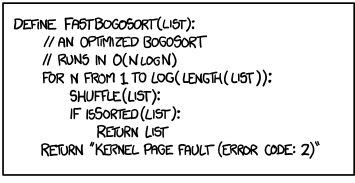
\includegraphics[width=300px]{fastbogosort.png}
    \label{fig:fastbogosort}
  \end{figure}
  \begin{itemize}
  \item Quelle: \url{http://xkcd.com/1185/}
  \end{itemize}
\end{frame}

\begin{frame}
  \frametitle{"Uberblick Tutorium}
  \begin{itemize}
  \item Algorithmenanalyse
    \begin{itemize}
    \item Laufzeitanalyse
      \begin{itemize}
      \item RAM-Modell
      \item Landau-Symbole
      \end{itemize}
    \item Korrektheitsbeweise: Schleifeninvarianten
    \end{itemize}
  \item (Algorithmenentwurf)
    \begin{itemize}
    \item Divide \& Conquer
    \end{itemize}
  \item Aktuelles "Ubungsblatt
  \end{itemize}
\end{frame}

\section{Laufzeitanalyse}
\subsection{Grundlagen/RAM-Modell}
\begin{frame}
  \frametitle{Laufzeitanalyse}
  \begin{itemize}
  \item Ziel: Konkrete Aussagen "uber Laufzeit eines Algorithmus,
        in Abh"angigkeit der Eingabegr"o"se (mathematische Funktion!)
  \item Stufe verschiedene Eingabetypen ein:
    \begin{itemize}
    \item \textbf{Worst case}: Familie von Eingaben, bei denen der Algorithmus
          besonders viel Laufzeit erfordert
    \item \textbf{Best case}: Familie von Eingaben, bei denen der Algorithmus
          besonders schnell fertig wird (meist uninteressant)
    \end{itemize}
  \item Im Folgenden Untersuchung der \textbf{Worst-Case-Laufzeit}
  \item Idee: Z"ahlen von Operationen in einem geeigneten Rechnermodell
    \begin{itemize}
    \item \textbf{RAM-Modell}: Speicherzugriffe und arithmetische Operationen
          ben"otigen konstante Zeit
    \end{itemize}
  \end{itemize}
\end{frame}

\begin{frame}[fragile]
  \frametitle{Laufzeitanalyse (Beispiel)}
  \begin{itemize}
  \item Eingabe: Array \emph{array} der Gr"o"se $n$
  \item Ausgabe: \visible<2->{FALSE, falls $array$ doppeltes Element enth"alt, sonst TRUE}
  \end{itemize}
  \begin{lstlisting}
  Function %*\visible<2->{UNIQUE}*)(array, x)
      for i := 0 to array.length - 1
          for j := i + 1 to array.length - 1
              if array[i] = array[j]
                  return FALSE
      return TRUE
  \end{lstlisting}
  \begin{itemize}
  \item Was macht dieser Algorithmus?
  \visible<2->{
  \item Was sind die Worst-Case-Eingaben?
  \item Wie viele Operationen werden im \emph{worst case} ausgef"uhrt?
  \end{itemize}
  }
\end{frame}

\subsection{Landau-Symbole}
\begin{frame}
  \frametitle{Landau-Symbole}
  \begin{itemize}
  \item Machen Aussagen "uber \textbf{asymptotisches Wachstum} von Funktionen
  \item Konstante Faktoren werden ignoriert
    \begin{itemize}
    \item Oft Implementierungsdetail, Kompensation durch
          bessere Programmiersprachen/Mikrooptimierung/Hardware
    \end{itemize}
  \item Endlich viele Funktionswerte k"onnen ignoriert werden
    \begin{itemize}
    \item Vor allem gro"se $n$ sind interessant
    \end{itemize}
  \item Beispiel: $f(n) = \frac{5}{2}n^2 + \frac{1}{2}n$ verh"alt sich f"ur gen"ugend gro"ses
        $n$ bis auf Faktor $\frac{5}{2}$ wie $g(n) = n^2$, wir wollen
        Zusammenhang ausdr"ucken k"onnen \\[1em]
          $\rightarrow f(n) = \Theta(n^2)$
 %\begingroup
%\setbeamercolor{block title}{bg=red,fg=blue}%bg=background, fg= foreground
%\setbeamercolor{block body}{bg=yellow,fg=green}%bg=background, fg= foreground
 %\begin{definition}
   %A group $G$ is cyclic if there existis an element $x\in G$ such that $\langle x\rangle=G$.
 %\end{definition}
%\endgroup
  \end{itemize}
\end{frame}

\begin{frame}
  \frametitle{Landau-Symbole (2)}
  \begin{itemize}
  \item $f \in \bigO(g) \iff$ $f$ ,,w"achst h"ochstens so schnell wie'' $g$
      \[\visible<2->{\textcolor{red}{\exists c > 0}} \ \
        \visible<3->{\textcolor{blue}{\exists n_0}} \quad
        f(n) \leq \visible<2->{\textcolor{red}{c\cdot}} g(n) \ \
        \forall n \ \visible<3->{\textcolor{blue}{\geq n_0}}\]
  \visible<4->{
  \item $f \in \Omega(g) \iff$ $f$ ,,w"achst mindestens so schnell wie'' $g$

      \[\visible<5->{\textcolor{red}{\exists c > 0}} \ \
        \visible<6->{\textcolor{blue}{\exists n_0}} \quad
        f(n) \geq \visible<5->{\textcolor{red}{c\cdot}} g(n) \ \
        \forall n \ \visible<6->{\textcolor{blue}{\geq n_0}}\]
  }
  \visible<7->{
  \item $f \in \Theta(g) \iff f \in \bigO(g) \text{ und } g \in \bigO(f)$
  }
  \visible<8->{
  \item h"aufig auch $f = \bigO(g)$ anstatt $f \in \bigO(g)$ etc.
  }
  \visible<9->{
  \item Auch in Termen m"oglich:
    \begin{align*}
        &T(n) = 2\cdot T\left(\frac{n}{3}\right) + \bigO(n) \\
        \visible<10->{
        \iff \visible<11->{\textcolor{red}{\exists c > 0}} \ \
          \visible<12->{\textcolor{blue}{\exists n_0}} \quad
          &T(n) \leq 2\cdot T\left(\frac{n}{3}\right) +
          \visible<11->{\textcolor{red}{c\cdot}} n \ \
          \visible<12->{\textcolor{blue}{\forall n \  \geq n_0}}
        }
    \end{align*}
  }
  %\item $f(n) = o(g(n))$
  %\item $f(n) = \omega(g(n))$
  \end{itemize}
\end{frame}

\begin{frame}
  \frametitle{Landau-Symbole (3)}
  \begin{itemize}
  \item $f \in o(g) \iff f \in \bigO(g) \setminus \Theta(g) \iff$
          $f$ ,,w"achst langsamer als'' $g$
      \[\lim_{n\rightarrow \infty} \frac{f(n)}{g(n)} = 0\]
  \visible<2->{
  \item $f \in \omega(g) \iff f \in \Omega(g) \setminus \Theta(g) \iff$
          $f$ ,,w"achst schneller als'' $g$
      \[\lim_{n\rightarrow \infty} \frac{f(n)}{g(n)} = \infty\]
  }
  \end{itemize}
\end{frame}

\begin{frame}
  \frametitle{Landau-Symbole (\emph{Cheat sheet})}
  \begin{center}
  \begin{tabular}{| l || l | l |} \hline
  \textbf{Notation} & \textbf{$f$ w"achst $\ldots$ $g$} & \textbf{Definition} \\ \hline
  $f \in o(g)$
      & echt langsamer als
      & $\lim_{n\rightarrow \infty} \frac{f(n)}{g(n)} = 0$
      \\ \hline
  $f \in \bigO(g)$
      & \footnotesize h"ochstens so schnell wie \normalsize
      & $\textcolor{red}{\exists c > 0}: \
          f(n) \leq \textcolor{red}{c\cdot} g(n) \textcolor{blue}{\text{ ffa } n}$
      \\ \hline
  $f \in \Theta(g)$
      & genauso schnell wie
      & \footnotesize $\textcolor{red}{\exists c_1, c_2 > 0}:
        \ \textcolor{red}{c_1\cdot} f(n)
            \leq g(n)
            \leq \textcolor{red}{c_2 \cdot} f(n)
          \textcolor{blue}{\text{ ffa } n}$ \normalsize
      \\ \hline
  $f \in \Omega(g)$
      & \footnotesize mindestens so schnell wie \normalsize
      & $\textcolor{red}{\exists c > 0}: \ f(n) \geq c\cdot g(n) \textcolor{blue}{\text{ ffa } n}$
      \\ \hline
  $f \in \omega(g)$
      & echt schneller als
      & $\lim_{n\rightarrow \infty} \frac{f(n)}{g(n)} = \infty$
      \\ \hline
  \end{tabular}
  \end{center}
  \begin{itemize}
  \item $o(g) \subset \bigO(g)$, $\omega(g) \subset \Omega(g)$
  \item $\Theta(g) = \bigO(g) \cap \Omega(g) = \{ f:\ f \in \bigO(g) \wedge g \in \bigO(f)\}$
  \item Insbesondere: $\Theta(g) \subset \bigO(g)$, $\Theta(g) \subset \Omega(g)$
  \end{itemize}
\end{frame}

\section{Korrektheitsbeweise}
\subsection{Grundlagen}
\begin{frame}[fragile]
  \frametitle{Linearsuche}
  \begin{itemize}
  \item Eingabe: Array \emph{array} der Gr"o"se $n$ und Element $x$
  \item Ausgabe: Index $i \in \{0,\ldots,n-1\}$ mit $\text{\emph{array}}[i] = x$
                 oder ,,not found'', falls das Element nicht im Array existiert
  \end{itemize}
  \begin{lstlisting}
  Function LINEAR-SEARCH(array, x)
      for i := 0 to array.length - 1
          if x = array[i]
              return i
      return "not found"
  \end{lstlisting}
\end{frame}

\begin{frame}[fragile]
  \frametitle{Bin"are Suche}
  \begin{itemize}
  \item Eingabe: Array \emph{array} der Gr"o"se $2^k$ mit $k \geq 1$ und Element
                 $x \in \text{\emph{array}}$. \\
                 \emph{array} sei aufsteigend sortiert und enthalte
                 keine doppelten Elemente
  \item Ausgabe: Index $i \in \{0,\ldots,2^k-1\}$ mit $a[i] = x$
  \end{itemize}
  \begin{lstlisting}
  Function BINARY-SEARCH(array, x)
      l := 0
      r := array.length    // = %*$\color{colcomment}{2^k}$*)
      while r - l > 1
          m := %*$\frac{1}{2}\left(l+r\right)$*)
          if x %*$\leq$*) array[m]
              r := m
          else
              l := m
      return l
  \end{lstlisting}
\end{frame}

\section{Algorithmenentwurf}
\subsection{Divide \& Conquer}
\begin{frame}
  \frametitle{Divide \& Conquer}
  \begin{itemize}
  \item Entwurfsprinzip ,,Teile und herrsche''
  \item Schritte:
    \begin{itemize}
    \item Zerlege Problem in $a$ Teilprobleme der Gr"o"se $\frac{n}{b}$
    \item L"ose Teilprobleme rekursiv
    \item F"uge Teilergebnisse zusammen in $\bigO(f(n))$
    \end{itemize}
  \item Laufzeit als \emph{Rekurrenz} formuliert:
    \[T(n) = a\cdot T\left(\frac{n}{b}\right) + \bigO(f(n))\]
  \item Ausblick: Master-Theorem liefert L"osung der Gleichung, also Laufzeitklasse von
        $T$
  \end{itemize}
\end{frame}

\begin{frame}
  \frametitle{Beispiel Divide \& Conquer: \\ Schnelles Potenzieren}
  \begin{itemize}
  \item Gegeben: Zahl $x$, Exponent $n \in \mathbb{N}_0$
  \item Gesucht: $x^n$
  \item Naiver Ansatz: Schleife "uber $n$, ben"otigt $\Omega(n)$ Multiplikationen
  \visible<2->{\item Das geht viel besser! Ideen?}
  \visible<3->{
  \item Beobachtung:
    \begin{align}
    x^{2k} &= \left(x^k\right)^2 \\
    x^{2k+1} &= \left(x^k\right)^2 \cdot x
    \end{align}
  \item Also: 1 Teilproblem der Gr"o"se $\frac{n}{2}$
  \item Zusammenf"ugen mit $\leq 2$ Multiplikationen in
         \[\rightarrow \text{ Anzahl Multiplikationen }
           M(n) = M\left(\frac{n}{2}\right) + \bigO(1) = \bigO(\log n)\]
  }
  \end{itemize}
\end{frame}

\end{document}
